\section{Technologies}

The software architecture determines not only the structure of the software, but it also helps in defining which type of technologies might be needed to build the system as efficiently as possible. Different technologies have their own advantages and disadvantages, and the goal of this phase is not to find the best technology or the best programming language, but rather to find the most suitable set of technologies given the priorities of the project and preferences of the writer.
From the software architecture diagram listed on \autoref{fig:sw-arc}, the technologies to be used on the following components should be defined:
\begin{itemize}
 \item User interface (web application)
 \item FDS (server-side application)
 \item Message broker / notification system 
 \item Database and caching memory
\end{itemize}

\begin{figure}[h]
 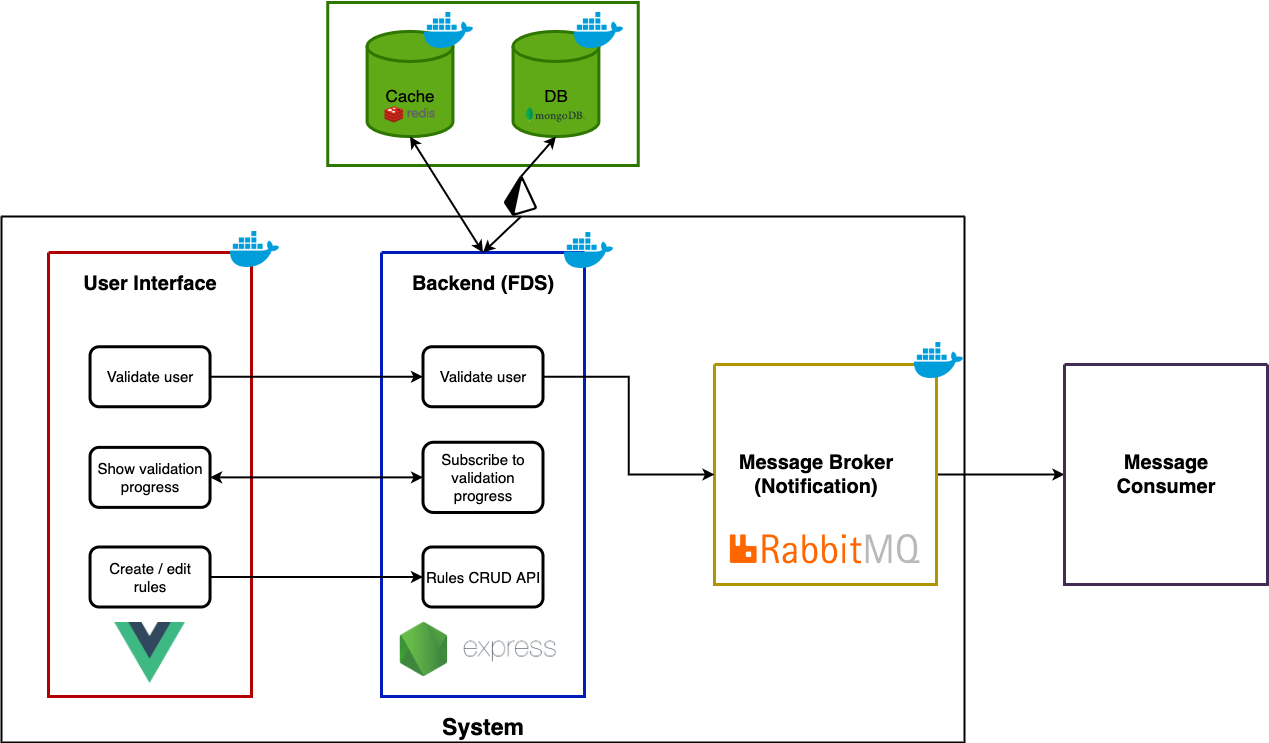
\includegraphics[width=\textwidth]{diagrams/architecture.png}
 \caption{Software architecture diagram with technologies used}
 \label{fig:sw-arc-tech}
\end{figure}

The previous software architecture diagram is therefore extended with additional logos of the technology used for each component of the system. All internal components of the system should be run as a Docker\footnote{\emph{Docker} is an open source software used to containerize applications in a package with its dependencies and operating system, making it runnable in any environment. Homepage: https://www.docker.com/.} container. Running the applications as a Docker container means that each application is started and run in isolation, ensuring portability to other operating systems. The database and caching memory will also be run as a Docker container, to avoid the need of installing the dependencies needed and to enable the possibility to start all the components of the system using a single command with Docker Compose\footnote{\emph{Docker Compose} is an open source tool for running multiple Docker containers. GitHub repository: \url{https://github.com/docker/compose}.}.

 \subsection{User Interface}
  \label{concept_ui}

 The technology used to build the user interface is VueJS (3. Version, also known as \emph{Vue3})\footnote{\emph{Vue3} is an open source JavaScript framework to build user interfaces. GitHub repository: \url{https://github.com/vuejs/core}.}, a JavaScript framework built on top of HTML, CSS and JavaScript for building a reactive user interfaces using a component-based programming paradigm. To ensure type safety, the user interface is built with TypeScript\footnote{\emph{TypeScript} is an open source programming language built by Microsoft on top of JavaScript by adding additional optional static typing. A TypeScript program will be compiled to a plain JavaScript program, before being executed in environment such as browser or NodeJS environment. GitHub repository: \url{https://github.com/microsoft/TypeScript}.}, rather than plain JavaScript, which is also supported by Vue3.

 \subsection{FDS}
  \label{concept_fds}

 The technology chosen to build the FDS is Node.JS\footnote{\emph{Node.JS} is an open source JavaScript runtime environment that runs on Google's V8 engine, enabling JavaScript programs to be run out of the browser environment. GitHub repository: \url{https://github.com/nodejs/node}.}. Node.JS is chosen not only because the writer is familiar with it, but also the event loop architecture of Node.JS enables the possibility to perform non-blocking I/O operations asynchronously. Each validation process will be an asynchronous process, which wouldn't block the main thread of the application. To ensure type safety, TypeScript is also used here rather than plain JavaScript. Express.JS\footnote{\emph{Express JS} is an open source web application framework for Node.JS. GitHub repository: \url{https://github.com/expressjs/expressjs.com}.} is the web framework of choice to build the FDS. Express.JS provides a simple and declarative API to build a web application with ease and speed.
An object-relational mapping tool (ORM) is used in this application to provide an easier access to the database, and additionally to keep the database schema in sync between the database server and the FDS application. The ORM of choice for the application is Prisma\footnote{\emph{Prisma} is an open source ORM for Node.JS and TypeScript. GitHub repository: \url{https://github.com/prisma/prisma}.}, as it provides a straightforward integration with TypeScript, generating TypeScript types automatically from the database schema.

 \subsection{Message Broker / Notification System}
 A reliable message broker is needed to make sure that all validation results actually reach every consumer. The technology chosen for this component is RabbitMQ\footnote{RabbitMQ is a messaging broker, enabling the distribution of messages across multiple clients. RabbitMQ homepage: \url{https://www.rabbitmq.com/}.}, as it is not only reliable, but also has an easy guide to set up as well as a big collection of client libraries for multiple programming languages.

 \subsection{Database and Caching Memory}
 A database is needed to store data regarding validation rules. Each database system has their own use cases and weaknesses. For this particular project, MongoDB\footnote{\emph{MongoDB} is a source-available NoSQL database developed by MongoDB Inc. MongoDB homepage: \url{https://www.mongodb.com/}.} will be used as the database system of choice. Redis\footnote{\emph{Redis} is an open-source in-memory data structure store. GitHub repository: \url{https://github.com/redis/redis}.} is chosen as the technology of choice for the caching memory because of its simple API and reliability. 